\documentclass[10pt,twocolumn]{article}
\usepackage[letterpaper,margin=0.7in,columnsep=0.25in]{geometry}
\usepackage[T1]{fontenc}
\usepackage{amsmath}
\usepackage{mathptmx}
\usepackage[dvipsnames]{xcolor}
\usepackage{graphicx,booktabs,multirow}
\usepackage[font=small,labelfont=bf]{caption}
\usepackage[round,authoryear]{natbib}
\usepackage[colorlinks=true,linkcolor=blue!50!black,citecolor=blue!50!black,urlcolor=blue!50!black]{hyperref}
\usepackage{enumitem}
\setlist{nosep,leftmargin=*}
\setlength{\bibsep}{1pt}
\renewcommand{\bibfont}{\footnotesize}

\title{\vspace{-1.2em}\textbf{Benchmarking Machine-Learning Models for PAM50 Intrinsic Subtype Classification Using TCGA-BRCA Gene Expression Data}}
\author{Ceaser Kaiwusaier\\[2pt]
\small Advanced Bioinformatics I, Section 01 --- Instructor: Xiangyu Li, Ph.D.\\
\small School of Computer Science and Engineering, California State University, San Bernardino --- Fall 2026\\[2pt]
\small Video presentation: \url{[VIDEO-LINK]} \quad Code: \url{https://github.com/Ceaser0927/pam50-benchmark}}
\date{\vspace{-2em}}

\begin{document}
\twocolumn[
\maketitle
\begin{abstract}
\noindent Breast cancer comprises molecularly distinct intrinsic subtypes whose identification guides prognosis and treatment, and the 50-gene PAM50 signature is the standard tool for assigning them. Machine-learning classifiers are increasingly applied to such expression data, but it is unclear whether flexible nonlinear models add anything when the input is already a small, biologically curated gene set. We benchmarked multinomial logistic regression against three nonlinear classifiers---random forest, RBF-kernel support vector machine and XGBoost---for reproducing PAM50 labels from the expression of the 50 PAM50 genes in 844 TCGA-BRCA primary tumours. All models were tuned by repeated stratified cross-validation inside leakage-safe pipelines and evaluated once on a held-out test set with bootstrap confidence intervals and paired statistical comparisons. Logistic regression achieved the highest cross-validated and held-out balanced accuracy (0.92 and 0.89); no nonlinear model significantly outperformed it, and random forest and XGBoost were significantly worse in cross-validation. For every model, most errors were Luminal A/Luminal B confusions, and the most useful genes mapped onto the known oestrogen-receptor, HER2-amplicon and basal-keratin programmes. Within a fixed PAM50 feature space, subtype information is captured by an essentially linear structure, and added model complexity provides no measurable benefit.
\end{abstract}
\vspace{1em}]

\section{Introduction}
Breast cancer is not a single disease. Gene-expression profiling revealed reproducible ``intrinsic'' subtypes---Luminal A, Luminal B, HER2-enriched, Basal-like and Normal-like---that differ in cell of origin, mutational landscape, prognosis and response to endocrine, anti-HER2 and cytotoxic therapy \citep{perou2000,sorlie2001,prat2011}. \citet{parker2009} distilled these subtypes into the 50-gene PAM50 assay, which assigns a tumour to the subtype whose expression centroid it correlates with most strongly. The Cancer Genome Atlas (TCGA) later profiled more than one thousand breast tumours and used PAM50 to organise its multi-omic findings \citep{tcga2012}, making TCGA-BRCA the reference public dataset for subtype research.

Subtype assignment is nonetheless imperfect. Single-sample predictors disagree for a sizeable fraction of tumours, and the boundary between the two luminal subtypes, which is defined largely by proliferation rather than by a qualitative switch, is the least stable \citep{weigelt2010}. Methods such as PCA-PAM50 have tried to improve consistency by changing how samples are normalised, and they reclassify a subset of Luminal A tumours as Luminal B \citep{paquet2019}. At the same time, nonlinear machine-learning models such as random forests and gradient-boosted trees are increasingly applied to expression data on the premise that they capture gene--gene interactions that simpler models miss. Whether that premise holds for a small, deliberately chosen feature set is rarely tested under controlled conditions. In clinical prediction more broadly, flexible models frequently fail to beat logistic regression \citep{christodoulou2019}.

This project addresses that gap with a controlled benchmark. We ask: \emph{with the feature set fixed to the PAM50 genes, do nonlinear classifiers reproduce PAM50 subtype labels meaningfully better than a linear model?} Fixing the features removes feature selection as a confounder, so any difference reflects the learning algorithm alone. We additionally ask which subtypes are hardest to separate---in particular whether Luminal A and B are confused---and which genes the models rely on. Section~\ref{sec:methods} describes the data and the evaluation design, Section~\ref{sec:results} presents the comparison, and Section~\ref{sec:discussion} interprets the findings and their limitations.

\section{Methods}\label{sec:methods}
\subsection{Data and cohort construction}
We downloaded two files from the UCSC Xena TCGA Hub \citep{goldman2020}, cohort \textit{TCGA Breast Cancer (BRCA)}, on 24 November 2026. The first, \texttt{TCGA.BRCA.sampleMap/HiSeqV2}, contains gene-level Illumina HiSeq RNA-seq expression as $\log_2(\text{RSEM normalised count}+1)$ \citep{li2011} for 20,530 genes and 1,218 samples. The second, \texttt{TCGA.BRCA.sampleMap/BRCA\_clinicalMatrix}, contains phenotypes for 1,247 samples and includes the RNA-seq PAM50 call (\texttt{PAM50Call\_RNAseq}). All 1,218 expression samples had a phenotype record. We applied four filters in order (Fig.~\ref{fig:pipeline}):
\begin{enumerate}
\item Keep primary tumours only (TCGA barcode sample-type code \texttt{01}), leaving 1,097 samples.
\item Keep samples with a PAM50 call in \{LumA, LumB, Her2, Basal, Normal\}, leaving 844 samples.
\item Keep one sample per patient; there were no duplicate patients.
\item Restrict the features to the 50 PAM50 genes \citep{parker2009}.
\end{enumerate}
The first filter is essential. Of the 119 samples labelled ``Normal'', 95 were adjacent normal tissue rather than tumour, so keeping them would have turned the Normal-like class into a tumour-versus-normal problem. All 50 PAM50 genes were present; \textit{ORC6} appeared under its former symbol \textit{ORC6L}. The final matrix had no missing values. The cohort comprised 421 Luminal A, 192 Luminal B, 141 Basal-like, 67 HER2-enriched and 23 Normal-like tumours (Fig.~\ref{fig:cohort}).

\begin{figure*}[t]
\centering
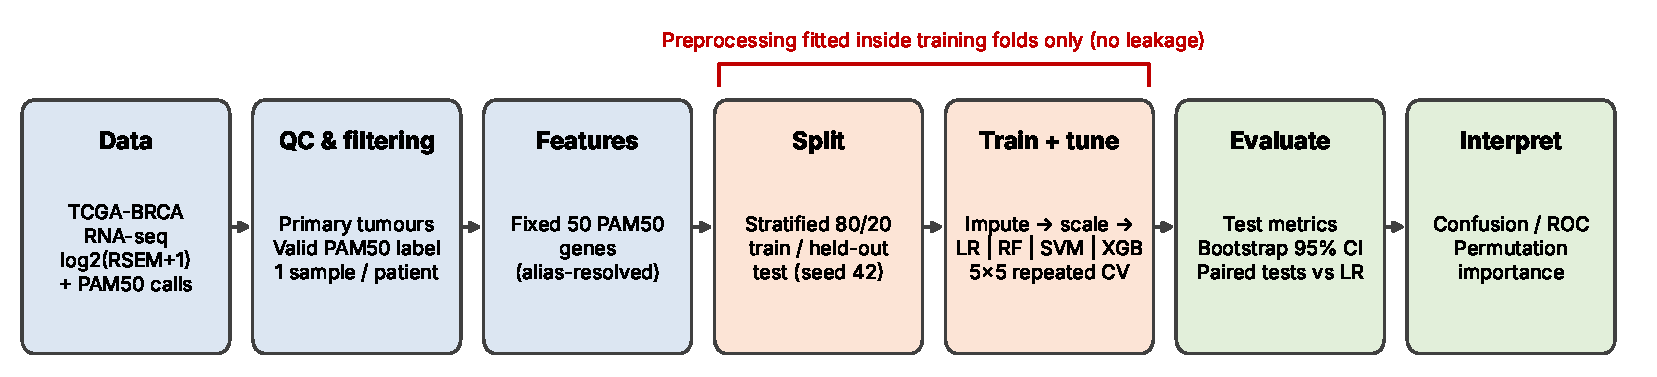
\includegraphics[width=\textwidth]{figures/fig0_pipeline.pdf}
\caption{Analysis workflow. Steps shaded orange use training data only. Imputation and standardisation sit inside every model pipeline and are re-fitted within each cross-validation fold, so neither validation folds nor the held-out test set influence preprocessing.}
\label{fig:pipeline}
\end{figure*}

\begin{figure}[t]
\centering
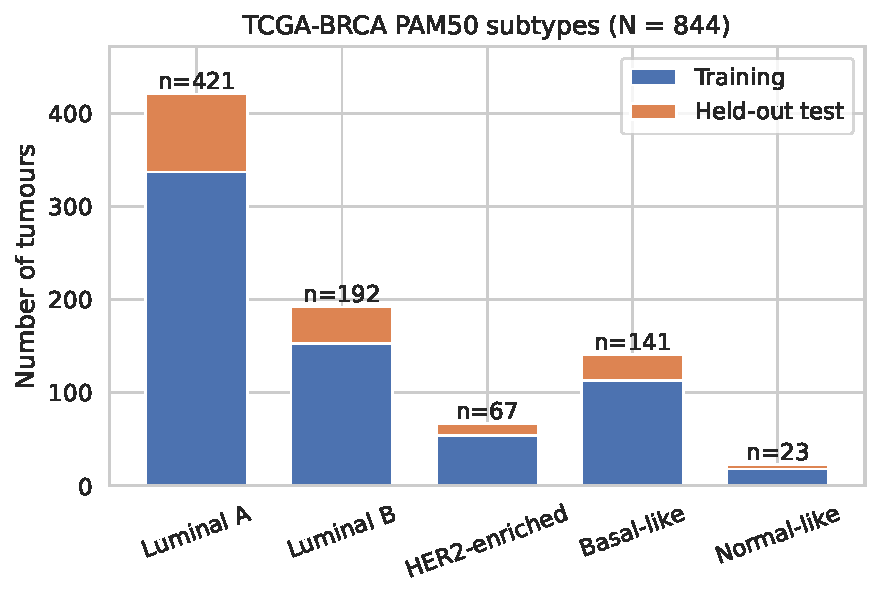
\includegraphics[width=\columnwidth]{figures/fig1_subtype_distribution.pdf}
\caption{PAM50 subtype distribution of the 844 analysed primary tumours and its stratified 80/20 partition. The roughly 18-fold imbalance between Luminal A and Normal-like motivates balanced class weights and class-averaged metrics.}
\label{fig:cohort}
\end{figure}

\subsection{Models and training}
The data were split once into a stratified training set (675 tumours) and a held-out test set (169 tumours) with seed 42. The test set was touched only for the final evaluation. Each model was implemented as a scikit-learn \citep{pedregosa2011} pipeline of median imputation, gene-wise standardisation and a classifier, so preprocessing was always fitted on training folds only. The four classifiers span increasing flexibility:
\begin{itemize}
\item \textbf{Multinomial logistic regression (LR)} with an L2 penalty. This is the linear baseline; its decision boundaries are hyperplanes in gene space.
\item \textbf{Random forest (RF)} \citep{breiman2001} with 500 trees. It averages deep decision trees that can represent arbitrary gene interactions.
\item \textbf{Support vector machine (SVM)} with an RBF kernel \citep{cortes1995}. It fits smooth nonlinear boundaries, and Platt scaling provides class probabilities.
\item \textbf{XGBoost} \citep{chen2016}, gradient-boosted trees with subsample and column-sample rates of 0.8. Its tree depth directly controls the order of the interactions it can learn.
\end{itemize}
Class imbalance was handled with balanced class weights (LR, RF, SVM) or balanced sample weights (XGBoost). Hyper-parameters were chosen by grid search over 5-fold $\times$ 5-repeat stratified cross-validation (25 folds) on the training set, maximising balanced accuracy. The grids were:
\begin{itemize}
\item LR: $C\in[10^{-4},10]$ (nine values);
\item RF: \texttt{max\_features} $\in$ \{\texttt{sqrt}, 0.3\} $\times$ \texttt{min\_samples\_leaf} $\in$ \{1, 3, 5, 10, 20\};
\item SVM: $C\in\{0.1,1,10,100\}$ $\times$ $\gamma\in\{\text{scale},10^{-2},10^{-3},10^{-4}\}$;
\item XGBoost: depth $\in\{1,2,4\}$ $\times$ learning rate $\in\{0.03,0.1,0.3\}$ $\times$ trees $\in\{100,200,400\}$.
\end{itemize}
An initial run placed several optima on grid edges, so the grids were widened before the final run; Table~\ref{tab:results} reports the selected values. All models used identical folds, which allows paired comparisons.

\subsection{Evaluation and statistics}
Because the classes are imbalanced, we report class-averaged metrics: balanced accuracy (mean per-class recall), macro precision, macro F1 and macro one-versus-rest ROC-AUC. Two complementary comparisons against the LR baseline were made:
\begin{itemize}
\item \textbf{Cross-validation.} The 25 paired fold-wise differences in balanced accuracy were tested with the corrected resampled $t$-test of \citet{nadeau2003}. This test inflates the variance to account for overlapping training sets; a naive paired $t$-test on cross-validation folds is anti-conservative.
\item \textbf{Held-out test set.} We drew 2,000 class-stratified bootstrap resamples \citep{efron1993} and reused the same resamples for every model. This gives 95\% percentile confidence intervals (CIs) for each metric and for each model's paired difference from LR.
\end{itemize}
Errors were examined with row-normalised confusion matrices. Gene contributions were estimated with permutation importance \citep{breiman2001} on the test set: the mean drop in balanced accuracy over 30 random permutations of each gene. All randomness was seeded. The analysis used Python 3.13 with NumPy 2.5 \citep{harris2020}, pandas 3.0 \citep{mckinney2010}, SciPy 1.18 \citep{virtanen2020}, scikit-learn 1.9.1, XGBoost 3.4.1, Matplotlib 3.11 \citep{hunter2007} and seaborn 0.13 \citep{waskom2021}. A complete run takes about 6~minutes on a 2-core x86-64 CPU with 8~GB of RAM and no GPU. Code, pinned dependencies and the exact train/test assignment are available in the repository.

\section{Results}\label{sec:results}
\subsection{Nonlinear models do not outperform logistic regression}
Table~\ref{tab:results} and Fig.~\ref{fig:perf} compare the models. In cross-validation, LR had the highest mean balanced accuracy (0.923) and the lowest variability across folds. The RBF-SVM was statistically indistinguishable from it (difference $-0.012$, corrected $p=0.35$). Both tree ensembles were significantly worse: RF by $-0.060$ ($p=0.030$) and XGBoost by $-0.071$ ($p=0.012$). Their fold-to-fold spread was also up to twice as large (Fig.~\ref{fig:perf}A), meaning they were less stable as well as less accurate.

The held-out test set reproduced the ranking: balanced accuracy was 0.894 for LR, 0.882 for SVM, 0.874 for RF and 0.865 for XGBoost. However, with 169 test tumours the 95\% CIs are wide (about $\pm0.07$) and overlap heavily (Fig.~\ref{fig:perf}B). The paired bootstrap differences from LR were all negative and none excluded zero:
\begin{itemize}
\item SVM: $-0.012$ [$-0.030$, 0.005];
\item RF: $-0.020$ [$-0.069$, 0.023];
\item XGBoost: $-0.029$ [$-0.077$, 0.015].
\end{itemize}
The only interval that excluded zero favoured LR (SVM macro F1, $-0.025$ [$-0.055$, $-0.002$]). Ranking quality was uniformly high: macro ROC-AUC was 0.982--0.986 for every model, with no paired difference distinguishable from zero. All models therefore order tumours almost equally well, and the differences arise from where their decision thresholds fall rather than from the information they extract.

A telling detail is the configuration XGBoost selected: trees of depth~1 (decision stumps), a learning rate of 0.03 and 400 rounds. A boosted ensemble of stumps is an additive model with no gene--gene interaction terms. Given the freedom to model interactions of order 2 or 4, cross-validation preferred none. Likewise, the SVM's selected $\gamma=10^{-3}$ produces a wide kernel whose boundaries are only gently curved. Overall, the evidence does not support the hypothesis that nonlinear models improve PAM50 classification; the simplest model was at least as good as any alternative.

\begin{table*}[t]
\centering
\caption{Model comparison. CV: mean $\pm$ SD of balanced accuracy over 25 folds (5$\times$5 repeated stratified CV, training set); $p$: Nadeau--Bengio corrected resampled $t$-test of the paired fold-wise difference from LR. Test: held-out set ($n=169$) with stratified-bootstrap 95\% CIs (2,000 resamples). Best value in each column in bold.}
\label{tab:results}
\small
\resizebox{\textwidth}{!}{%
\begin{tabular}{lccccccl}
\toprule
& \multicolumn{2}{c}{Cross-validation} & \multicolumn{4}{c}{Held-out test set} & \\
\cmidrule(lr){2-3}\cmidrule(lr){4-7}
Model & Bal.\ acc. & $p$ vs LR & Bal.\ acc. & Macro precision & Macro F1 & Macro ROC-AUC & Selected hyper-parameters\\
\midrule
Logistic regression & \textbf{0.923} $\pm$ 0.030 & --- & \textbf{0.894} [0.81, 0.95] & 0.809 [0.74, 0.90] & 0.841 [0.77, 0.91] & 0.983 [0.96, 1.00] & $C=0.03$\\
SVM (RBF) & 0.911 $\pm$ 0.028 & 0.35 & 0.882 [0.80, 0.94] & 0.780 [0.72, 0.87] & 0.816 [0.74, 0.89] & \textbf{0.986} [0.98, 0.99] & $C=1$, $\gamma=10^{-3}$\\
Random forest & 0.863 $\pm$ 0.050 & 0.030 & 0.874 [0.78, 0.95] & 0.806 [0.74, 0.90] & 0.830 [0.75, 0.91] & 0.985 [0.97, 0.99] & sqrt features, min.\ leaf 10\\
XGBoost & 0.852 $\pm$ 0.060 & 0.012 & 0.865 [0.77, 0.94] & \textbf{0.837} [0.76, 0.93] & \textbf{0.849} [0.76, 0.92] & 0.982 [0.97, 0.99] & depth 1, lr 0.03, 400 trees\\
\bottomrule
\end{tabular}}
\end{table*}

\begin{figure*}[t]
\centering
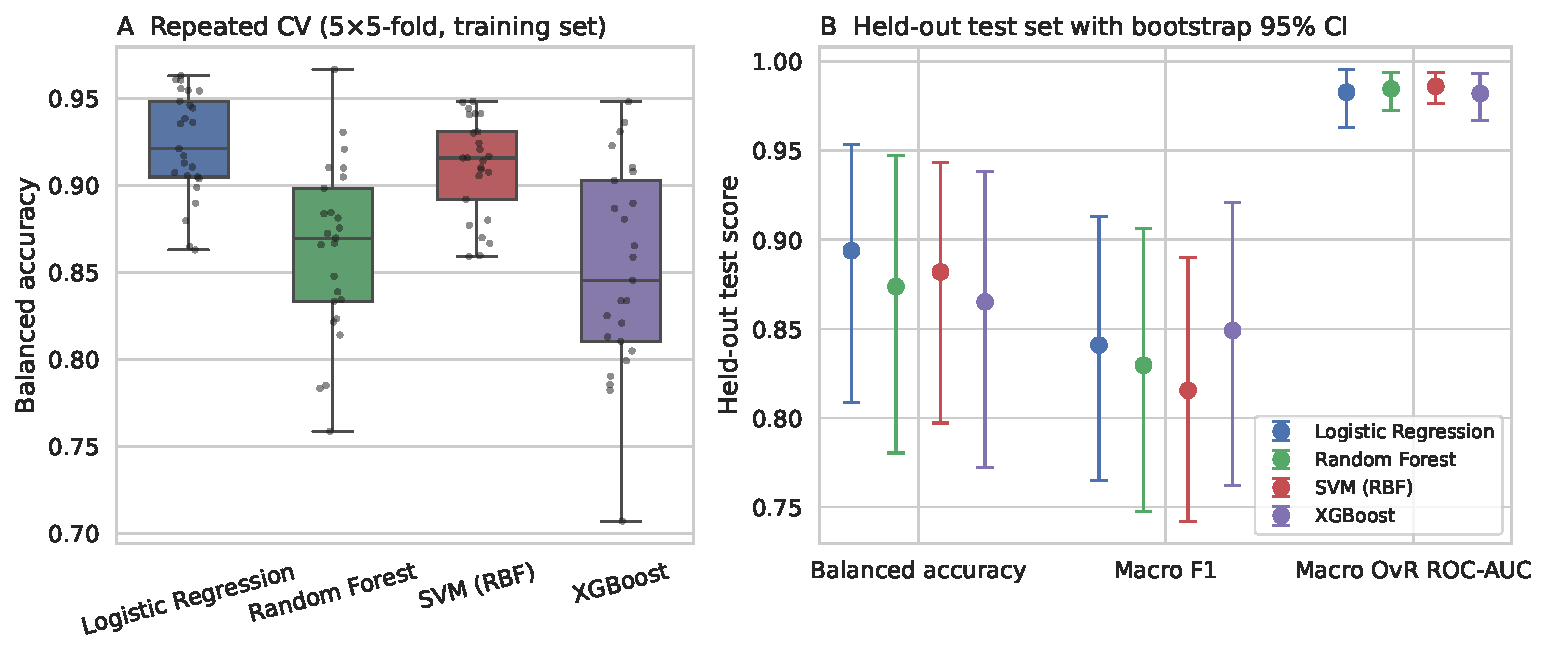
\includegraphics[width=0.92\textwidth]{figures/fig2_model_performance.pdf}
\caption{Model performance. (A) Balanced accuracy of the tuned models across the 25 cross-validation folds; folds are identical across models. (B) Held-out test scores with stratified-bootstrap 95\% CIs. Logistic regression is never significantly beaten; the tree ensembles are less accurate and more variable in cross-validation, and ROC-AUC is near-identical for all models.}
\label{fig:perf}
\end{figure*}

\subsection{Errors concentrate at the Luminal A/B boundary}
The confusion matrices (Fig.~\ref{fig:cm}) show that the models fail in the same places. Luminal A/B confusions accounted for 53--63\% of all test errors, depending on the model: 10 of 19 errors for LR, 11 of 20 for RF, 14 of 24 for SVM and 12 of 19 for XGBoost. The models differed mainly in which way they leaned. SVM and RF pushed Luminal A tumours into Luminal B (11 and 9 cases), whereas XGBoost erred symmetrically (6 each way). In contrast, Basal-like tumours were never confused with luminal tumours, and HER2-enriched recall was 0.85--1.00. Every model called two Basal-like tumours and one Normal-like tumour HER2-enriched. When all four algorithms make the same kind of error at the same rate, it more likely reflects borderline biology or label noise than an algorithm-specific weakness. The Normal-like class (5 test tumours) was recalled at 0.80 by all models but had the lowest precision (0.50--0.67), because a few Luminal A tumours were assigned to it. This single small class drives most of the gap between macro recall and macro precision in Table~\ref{tab:results}.

\begin{figure*}[t]
\centering
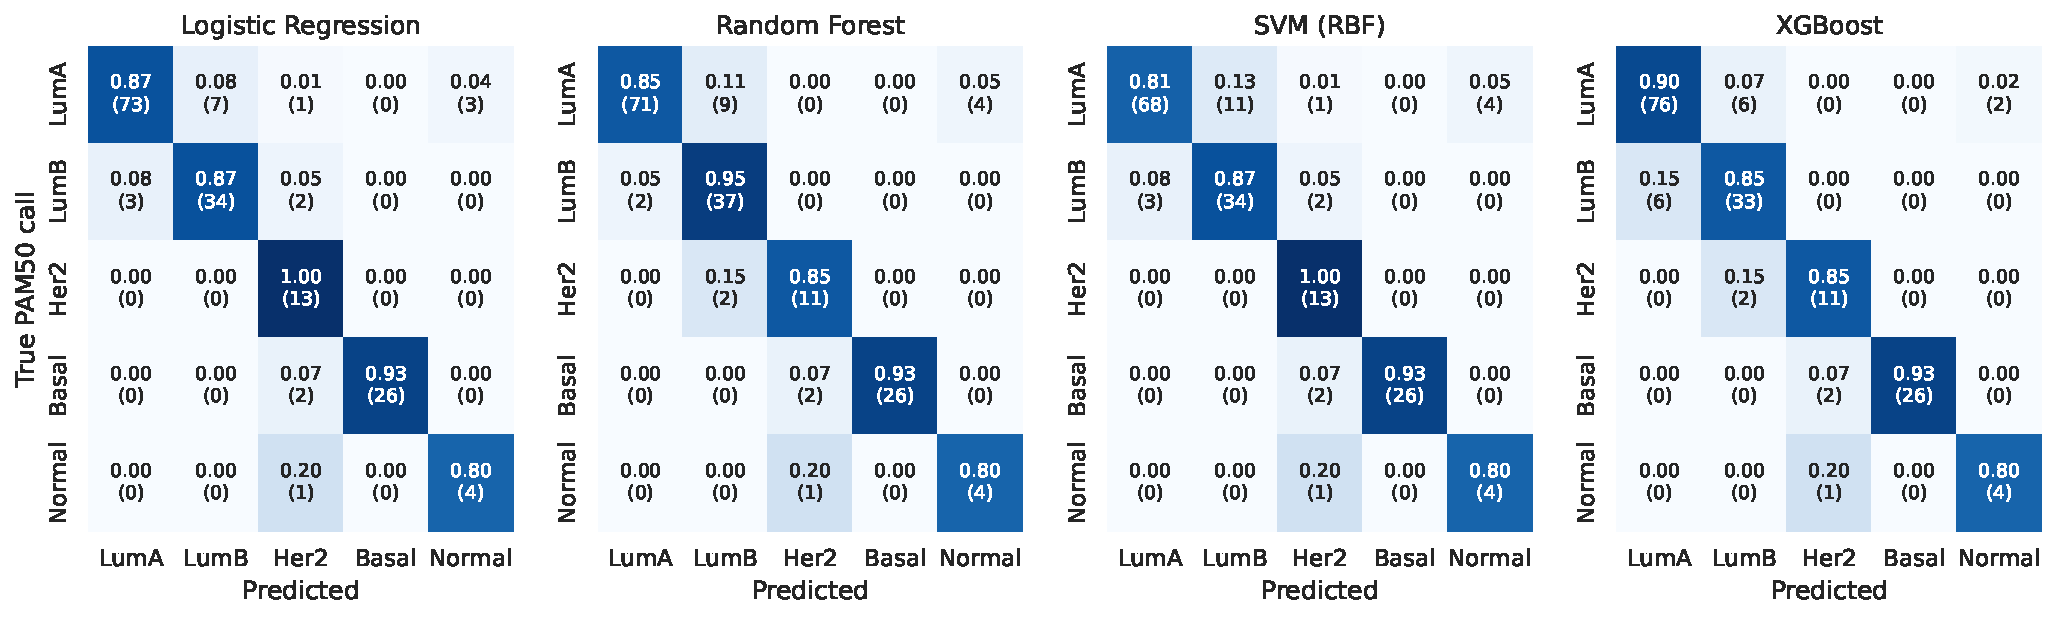
\includegraphics[width=\textwidth]{figures/fig3_confusion_matrices.pdf}
\caption{Row-normalised confusion matrices on the held-out test set (counts in brackets). Rows are TCGA PAM50 calls and columns are predictions. All four models make most of their errors between Luminal A and Luminal B, and never confuse Basal-like with luminal tumours.}
\label{fig:cm}
\end{figure*}

\subsection{Influential genes recover known subtype programmes}
Permutation importance (Fig.~\ref{fig:imp}) shows which genes the models' predictions depend on. Despite different exact rankings, the genes ranked highly by each model fall into three well-characterised programmes:
\begin{itemize}
\item \textbf{Oestrogen-receptor/luminal:} \textit{ESR1}, \textit{FOXA1}, \textit{NAT1}, \textit{SLC39A6}, \textit{MAPT}, \textit{BCL2}. These separate luminal from non-luminal tumours.
\item \textbf{HER2 amplicon:} \textit{ERBB2} and its co-amplified neighbour \textit{GRB7}. These define the HER2-enriched subtype.
\item \textbf{Basal/myoepithelial:} \textit{KRT5}, \textit{KRT17}, \textit{KRT14}, \textit{FOXC1}, \textit{CDH3}, \textit{SFRP1}, \textit{EGFR}. These mark Basal-like tumours.
\end{itemize}
Proliferation genes (\textit{EXO1}, \textit{CEP55}, \textit{UBE2T}, \textit{NUF2}) also appear. These are the genes that separate Luminal B from Luminal A \citep{parker2009,cheang2009}. All three programmes match the biology from which PAM50 was built.

The rankings were, however, unstable across models. For example, \textit{KRT5} ranked first for SVM but 50th for RF, and \textit{ERBB2} ranked first for LR but 16th for SVM. The reason is redundancy: PAM50 contains tightly correlated gene modules, so permuting one gene costs little when a correlated partner carries the same signal \citep{strobl2008}. The importance values therefore describe which \emph{programmes} each model uses rather than a unique ranking of individual genes, and they indicate predictive usefulness, not causal roles.

\begin{figure}[!htb]
\centering
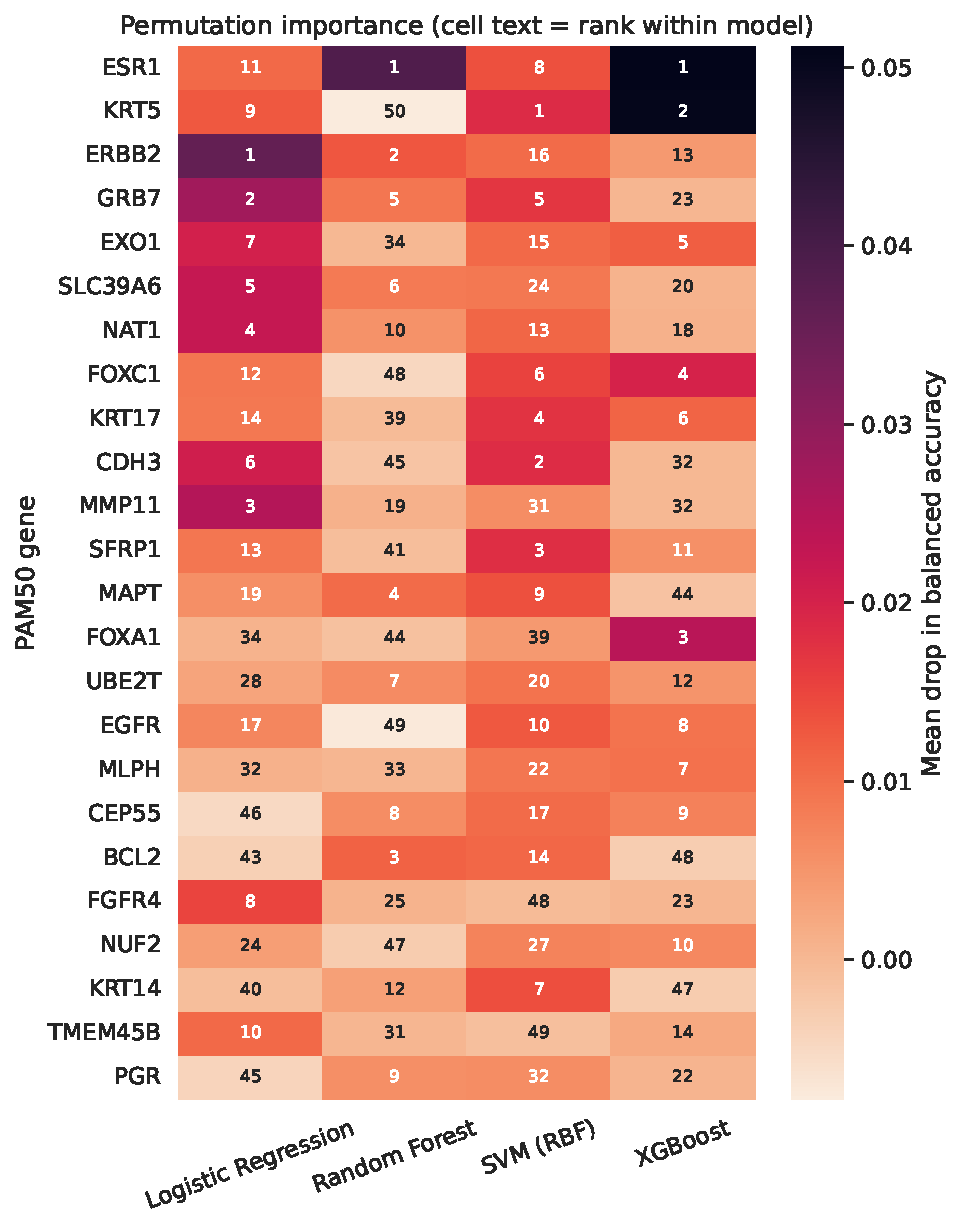
\includegraphics[width=0.82\columnwidth]{figures/fig5_permutation_importance.pdf}
\caption{Permutation importance on the test set (mean drop in balanced accuracy over 30 permutations) for the union of each model's top-10 genes; cell text gives the rank within each model. The top genes come from the ER/luminal, HER2-amplicon, basal-keratin and proliferation programmes, but exact ranks vary because correlated genes substitute for one another.}
\label{fig:imp}
\end{figure}

\section{Discussion}\label{sec:discussion}
The central finding is negative but informative. Once the input is restricted to the 50 PAM50 genes, a regularised linear model matches or exceeds random forests, kernel SVMs and gradient boosting. Three lines of evidence point the same way:
\begin{itemize}
\item LR ranked first in cross-validation and on the test set.
\item The tree ensembles were significantly worse and less stable in cross-validation.
\item When given the choice, XGBoost selected an interaction-free additive model.
\end{itemize}
This is consistent with how PAM50 was designed. The signature was chosen to separate subtypes by coordinated shifts in a few gene programmes, so the subtypes occupy distinct regions of PAM50 space that hyperplanes can separate well. In addition, the labels we predict were themselves produced by a nearest-centroid correlation rule \citep{parker2009,tcga2012}, whose decision boundaries are close to linear in standardised expression. The task therefore partly asks each model to recover a near-linear rule. Flexible models cannot gain from structure that is not present, and with only 18--54 training examples in the minority classes, their extra variance becomes a cost. This mirrors the broader observation that machine learning rarely beats logistic regression on structured, low-dimensional problems \citep{christodoulou2019}. In practical terms, the biologically curated signal matters more than algorithmic complexity.

The error analysis has a biological interpretation. Luminal A and B are not separated by a discrete event, such as the \textit{ERBB2} amplification that defines HER2-enriched tumours or the basal-keratin programme of Basal-like tumours. Instead they lie along a continuum of proliferation and oestrogen-receptor signalling \citep{cheang2009,prat2011}. Any classifier must place a threshold along that continuum, and tumours near it will be assigned inconsistently, which is the same instability documented for single-sample predictors \citep{weigelt2010} and addressed by PCA-PAM50 \citep{paquet2019}. That all four algorithms err at the same luminal and HER2 boundaries suggests the limit lies in the label definition rather than in model capacity. The weak Normal-like class fits the view that it partly reflects tumours with a large proportion of normal breast tissue rather than a distinct tumour biology \citep{prat2011}.

\textbf{Strengths.} The design isolates the effect of the algorithm:
\begin{itemize}
\item a fixed feature set;
\item identical folds for every model;
\item leakage-safe pipelines;
\item a single use of the test set;
\item statistics that respect the dependence between cross-validation folds;
\item paired bootstrap comparisons rather than visual comparison of point estimates.
\end{itemize}
The complete pipeline is seeded and reproducible from public data.

\textbf{Limitations.}
\begin{itemize}
\item \textbf{Circular labels.} The labels are computational PAM50 calls, not an independent ground truth, so we measure agreement with PAM50 rather than biological correctness. A nonlinear model could in principle capture biology that PAM50 itself misassigns, and this benchmark cannot detect that.
\item \textbf{Small test set.} With 169 test tumours, the CIs are wide enough that differences of about 0.03 in balanced accuracy cannot be resolved. Only 5 Normal-like test tumours make per-class estimates for that subtype anecdotal.
\item \textbf{Optimistic cross-validation scores.} The cross-validation scores are those of the selected configuration and are therefore slightly optimistic. Nested cross-validation would remove this bias, although it would apply equally to all models.
\item \textbf{One cohort and platform.} All results come from a single cohort and platform. Performance under batch effects or other normalisations (for example microarray cohorts such as METABRIC) is untested.
\item \textbf{Platt-scaled SVM probabilities.} Only the SVM's AUC depends on these probabilities, and they are approximate.
\end{itemize}

\textbf{Lessons and future directions.} The most consequential decisions in this project were about data handling rather than model choice. Recognising that most ``Normal'' labels belonged to normal tissue, and widening the hyper-parameter grids once edge optima appeared, mattered more than which classifier was used. Several follow-up experiments would strengthen the conclusions:
\begin{itemize}
\item \textbf{External validation.} Train on TCGA and test on an independent cohort such as METABRIC, to see whether flexible models degrade more under distribution shift.
\item \textbf{Independent labels.} Replace PAM50 calls with clinical endpoints (survival or treatment response) or with consensus labels, removing the circularity.
\item \textbf{Larger feature spaces.} Repeat the comparison on transcriptome-wide features, where nonlinear models and feature selection may matter more.
\item \textbf{Grouped importance.} Use grouped or conditional permutation importance to obtain stable, programme-level explanations.
\end{itemize}

\textbf{Conclusion.} For PAM50 subtype classification from PAM50 genes, model complexity is not the bottleneck. A simple, interpretable linear classifier is the appropriate choice, and remaining errors reflect the continuous biology of the luminal subtypes rather than missing nonlinear structure.

\bibliographystyle{plainnat}
\begin{thebibliography}{99}
\bibitem[Breiman(2001)]{breiman2001} Breiman, L. (2001). Random forests. \textit{Machine Learning}, 45(1), 5--32.
\bibitem[Cheang et~al.(2009)]{cheang2009} Cheang, M.C.U. et al. (2009). Ki67 index, HER2 status, and prognosis of patients with luminal B breast cancer. \textit{J. Natl. Cancer Inst.}, 101(10), 736--750.
\bibitem[Chen and Guestrin(2016)]{chen2016} Chen, T. and Guestrin, C. (2016). XGBoost: a scalable tree boosting system. In \textit{Proc. 22nd ACM SIGKDD}, pp. 785--794.
\bibitem[Christodoulou et~al.(2019)]{christodoulou2019} Christodoulou, E. et al. (2019). A systematic review shows no performance benefit of machine learning over logistic regression for clinical prediction models. \textit{J. Clin. Epidemiol.}, 110, 12--22.
\bibitem[Cortes and Vapnik(1995)]{cortes1995} Cortes, C. and Vapnik, V. (1995). Support-vector networks. \textit{Machine Learning}, 20(3), 273--297.
\bibitem[Efron and Tibshirani(1993)]{efron1993} Efron, B. and Tibshirani, R.J. (1993). \textit{An Introduction to the Bootstrap}. Chapman \& Hall, New York.
\bibitem[Goldman et~al.(2020)]{goldman2020} Goldman, M.J. et al. (2020). Visualizing and interpreting cancer genomics data via the Xena platform. \textit{Nat. Biotechnol.}, 38(6), 675--678. Data: \url{https://xenabrowser.net}, TCGA Hub, accessed 24 Nov 2026.
\bibitem[Harris et~al.(2020)]{harris2020} Harris, C.R. et al. (2020). Array programming with NumPy. \textit{Nature}, 585, 357--362.
\bibitem[Hunter(2007)]{hunter2007} Hunter, J.D. (2007). Matplotlib: a 2D graphics environment. \textit{Comput. Sci. Eng.}, 9(3), 90--95.
\bibitem[Li and Dewey(2011)]{li2011} Li, B. and Dewey, C.N. (2011). RSEM: accurate transcript quantification from RNA-Seq data with or without a reference genome. \textit{BMC Bioinformatics}, 12, 323.
\bibitem[McKinney(2010)]{mckinney2010} McKinney, W. (2010). Data structures for statistical computing in Python. In \textit{Proc. 9th Python in Science Conf.}, pp. 56--61.
\bibitem[Nadeau and Bengio(2003)]{nadeau2003} Nadeau, C. and Bengio, Y. (2003). Inference for the generalization error. \textit{Machine Learning}, 52(3), 239--281.
\bibitem[Paquet and Hallett(2019)]{paquet2019} Paquet, E.R. and Hallett, M.T. (2019). PCA-PAM50 improves consistency between breast cancer intrinsic and clinical subtyping reclassifying a subset of luminal A tumors as luminal B. \textit{Sci. Rep.}, 9, 7956.
\bibitem[Parker et~al.(2009)]{parker2009} Parker, J.S. et al. (2009). Supervised risk predictor of breast cancer based on intrinsic subtypes. \textit{J. Clin. Oncol.}, 27(8), 1160--1167.
\bibitem[Pedregosa et~al.(2011)]{pedregosa2011} Pedregosa, F. et al. (2011). Scikit-learn: machine learning in Python. \textit{J. Mach. Learn. Res.}, 12, 2825--2830.
\bibitem[Perou et~al.(2000)]{perou2000} Perou, C.M. et al. (2000). Molecular portraits of human breast tumours. \textit{Nature}, 406, 747--752.
\bibitem[Prat and Perou(2011)]{prat2011} Prat, A. and Perou, C.M. (2011). Deconstructing the molecular portraits of breast cancer. \textit{Mol. Oncol.}, 5(1), 5--23.
\bibitem[S{\o}rlie et~al.(2001)]{sorlie2001} S{\o}rlie, T. et al. (2001). Gene expression patterns of breast carcinomas distinguish tumor subclasses with clinical implications. \textit{Proc. Natl. Acad. Sci. USA}, 98(19), 10869--10874.
\bibitem[Strobl et~al.(2008)]{strobl2008} Strobl, C. et al. (2008). Conditional variable importance for random forests. \textit{BMC Bioinformatics}, 9, 307.
\bibitem[{The Cancer Genome Atlas Network}(2012)]{tcga2012} The Cancer Genome Atlas Network (2012). Comprehensive molecular portraits of human breast tumours. \textit{Nature}, 490, 61--70.
\bibitem[Virtanen et~al.(2020)]{virtanen2020} Virtanen, P. et al. (2020). SciPy 1.0: fundamental algorithms for scientific computing in Python. \textit{Nat. Methods}, 17, 261--272.
\bibitem[Waskom(2021)]{waskom2021} Waskom, M.L. (2021). seaborn: statistical data visualization. \textit{J. Open Source Softw.}, 6(60), 3021.
\bibitem[Weigelt et~al.(2010)]{weigelt2010} Weigelt, B. et al. (2010). Breast cancer molecular profiling with single sample predictors: a retrospective analysis. \textit{Lancet Oncol.}, 11(4), 339--349.
\end{thebibliography}
\end{document}
